\documentclass[]{standalone}
\usepackage{tikz}
\usepackage{pgfplots}

\begin{document}
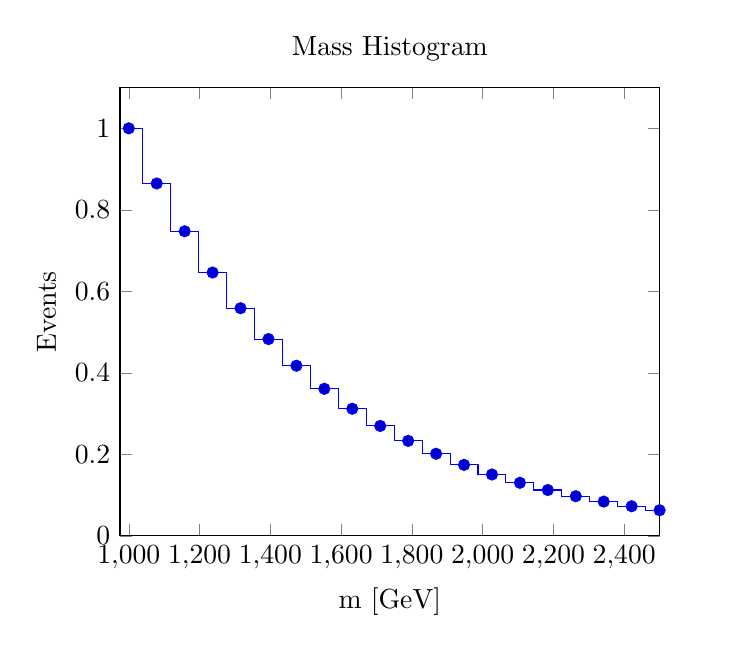
\begin{tikzpicture}
  \begin{axis}[
    ymin=0, ymax=1.1,
    xmin=975, xmax=2500,
    xlabel={m [GeV]},
    ylabel={Events},
    title=Mass Histogram,
    nodes near coords={\node (plot-\coordindex) at (axis cs:
\pgfkeysvalueof{/data point/x}, \pgfkeysvalueof{/data point/y}) {};}
    ]
    \addplot+[const plot mark mid, domain=1000:2500, samples=20] plot  {40^(-(x-1000)/2000)};
  \end{axis}
\end{tikzpicture}
\end{document}

